\chapter{Background and Literature}
\label{ch:background}

This chapter introduces technical concepts and background used in the conceptualized solution of the thesis. It also explains the state of the art of the different technologies used in the thesis and the current state of research in the field of sound source localization and distance estimation.

\section{Sound Propagation}

Sound propagation is the physical process by which sound waves propagate in a given environment. The strength of the sound wave is dependent on a variety of factors, including the frequency, environment, and distance from the sound source. This makes it difficult to accurately identify and localize a sound source, and thus a more accurate and robust sound source localization system is needed.

\subsection{Realistic sound propagation in simulations}

\subsection{Microsoft Project Acoustics}

Microsoft Project Acoustics is a sound propagation engine that simulates the propagation of sound waves in a given environment. It is used in a variety of applications, including video games, virtual reality, and augmented reality. It simulates wave effects like obstruction, reverberation and occlusion in complex 3D scenes without requiring zone markup or raytracing. It works similarly to a raytracing engine, but it is precomputed and optimized for real-time performance. 

\subsection{Sound Propagation in game-engine}

\section{Sound Source Localization}

Sound Source Localization (SSL) is the process of determining the position of a sound source. This is usually done using a microphone array that captures the sound signals from multiple directions. SSL is used in a variety of applications, such as speech recognition, robot navigation, surveillance, and security. In this thesis, SSL is used to estimate the distance and direction of a sound source to detect excessively noisy vehicles.

\subsection{Spectrograms for sound visualization}

Spectrograms are a visual representation of the frequency content of a sound signal. They are often used in sound source localization to identify the direction of a sound source. The spectrogram is a two-dimensional representation of the frequency content of a sound signal (figure \ref*{fig:spectrogram_example}).

\begin{figure}[H]
    \centering
    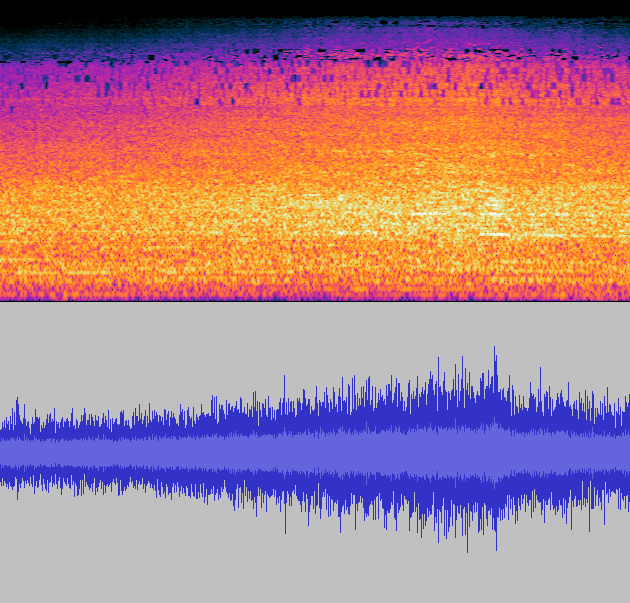
\includegraphics[width=0.5\textwidth]{../Images/spectrogram-example.png}
    \caption{Spectrogram of a sound signal}
    \label{fig:spectrogram_example}
\end{figure}

The x-axis represents time and the y-axis represents frequency. The intensity of the color at each point in the spectrogram represents the amplitude of the frequency component then. To represent multiple channels such as the ones recorded by a microphone array, the spectrogram is represented as a matrix of spectrograms, where each spectrogram represents the frequency content of a single channel (figure \ref*{fig:2_channel_spectrogram_example}).

\begin{figure}[H]
    \centering
    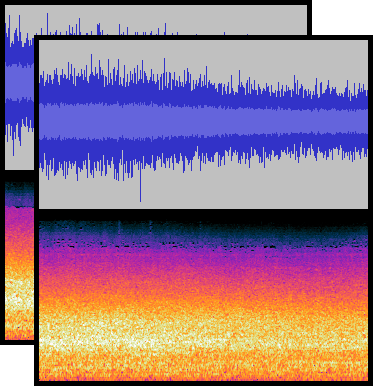
\includegraphics[width=0.4\textwidth]{../Images/2-channel-spectrogram-example.png}
    \caption{Dual channel spectrogram matrix of a sound signal}
    \label{fig:2_channel_spectrogram_example}
\end{figure}

The multi-channel spectrogram can be used to identify the time delta of a recorded sound by looking at the frequency content of the sound signal. The point in time where a sound is recorded will appear as a bright spot on the spectrogram and will determine the time of record. By comparing this time with the other channel, we can find the direction of the sound source. This is done by comparing the time delta of the sound signal with the time delta of the other channels (figure \ref*{fig:spectrogram_offset}).

\begin{figure}[H]
    \centering
    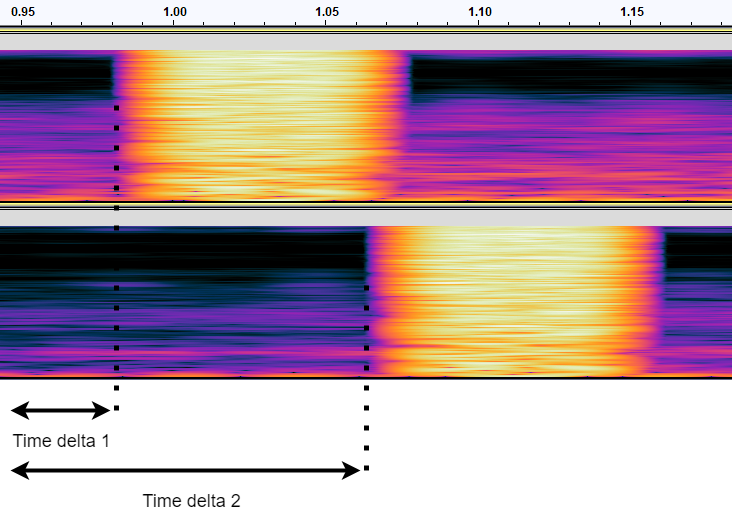
\includegraphics[width=0.5\textwidth]{../Images/time_delta.png}
    \caption{Spectrogram of two sound signals with time their delta}
    \label{fig:spectrogram_offset}
\end{figure}

Since we know the distance between the microphones, we can determine the direction of the sound.

\subsection{Origin of sound using two microphones}

Admitting the following setup (figure \ref*{fig:microphones_setup}), if the time delta 1 is greater than the time delta 2 of the other channels (setup 1) then the sound source is closer to the microphone 2. If the time delta 1 is equal to the time delta 2 (setup 3) then the sound source is equidistant to both microphones. If the time delta 2 is greater than the time delta 1 (setup 2) then the sound source is closer to the microphone 1. 

\begin{figure}[H]
    \centering
    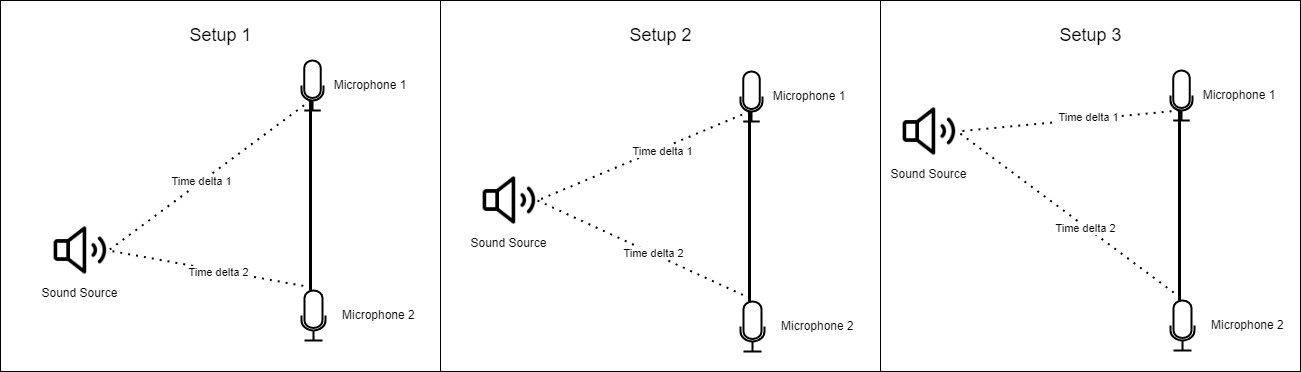
\includegraphics[width=1\textwidth]{../Images/microphones_setups.png}
    \caption{Sound source localization setup}
    \label{fig:microphones_setup}
\end{figure}

This can be formalized and is better explain in \cite{Scola2010DirectionOA}. Once the delay between the two microphones is known, the direction of the sound source can be found using trigonometric calculations. As in the figure \ref*{fig:sound-source-from-two-microphones}, considering point $M$ as the sound source and point $A$ and $B$ as microphones, the distance between the two microphones is $d$ and the time delta between the two microphones is $\Delta t$, the angle $\alpha$ can be calculated.

\begin{figure}[H]
    \centering
    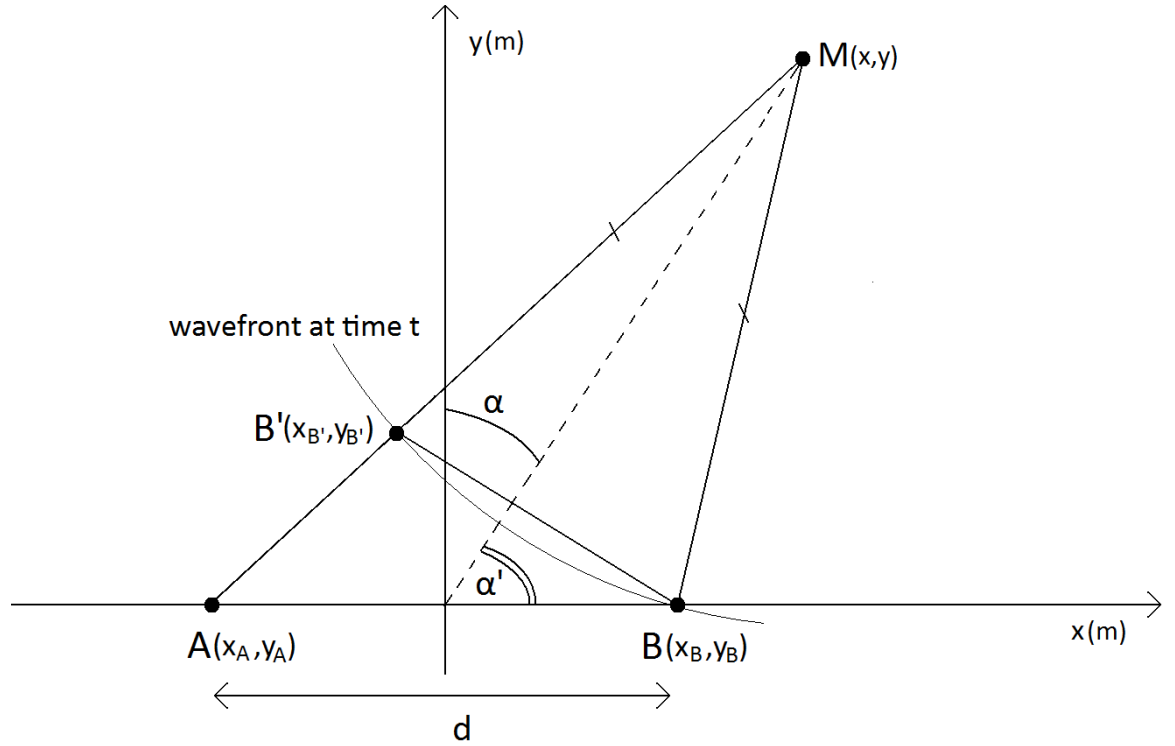
\includegraphics[width=0.7\textwidth]{../Images/sound-source-from-two-microphones.png}
    \caption{Sound source localization setup formalization. Original image from \cite{Scola2010DirectionOA}}
    \label{fig:sound-source-from-two-microphones}
\end{figure}

The following equation can be found:

\begin{equation}
    AB' = AM-B'M
\end{equation}

with Pythagorean theorem: 

\begin{equation}
    AM = \sqrt{(X_{a}-X)^2 + (Y_{a}-Y)^2}
\end{equation}
\begin{equation}
    BM = \sqrt{(X_{b}-X)^2 + (Y_{b}-Y)^2}
\end{equation}

The two microphones have the same $Y$ coordinate, so $Y_{a} = Y_{b} = Y$ and $Y_{a}-Y_{b} = 0$ and $X_{a} = -X_{B}$ The equation becomes:

\begin{equation}
    y = \pm\sqrt{\frac{AB'^2}{4} - x^2_{B} + x^2(\frac{4\cdot x^2_{B}}{AB'^2} - 1)}
\end{equation}

This setup shows that two microphones are enough to determine the direction of a sound source.
% TODO - compléter la formalisation

\section{Neural networks}

Neural networks are a type of machine learning algorithm based on a biological neuron that is used to solve a variety of problems, including image recognition, speech recognition, and natural language processing. Neural networks learn from provided data to solve a given problem without the need to explicitly program the solution. They are used in a variety of applications, including self-driving cars, facial recognition, and medical imaging. 

A neural network (figure \ref*{fig:neural_network}) is composed of multiple neurons (the circles) that are organized in layers and are connected to the neurons in the previous and next layers. 

\begin{figure}[H]
    \centering
    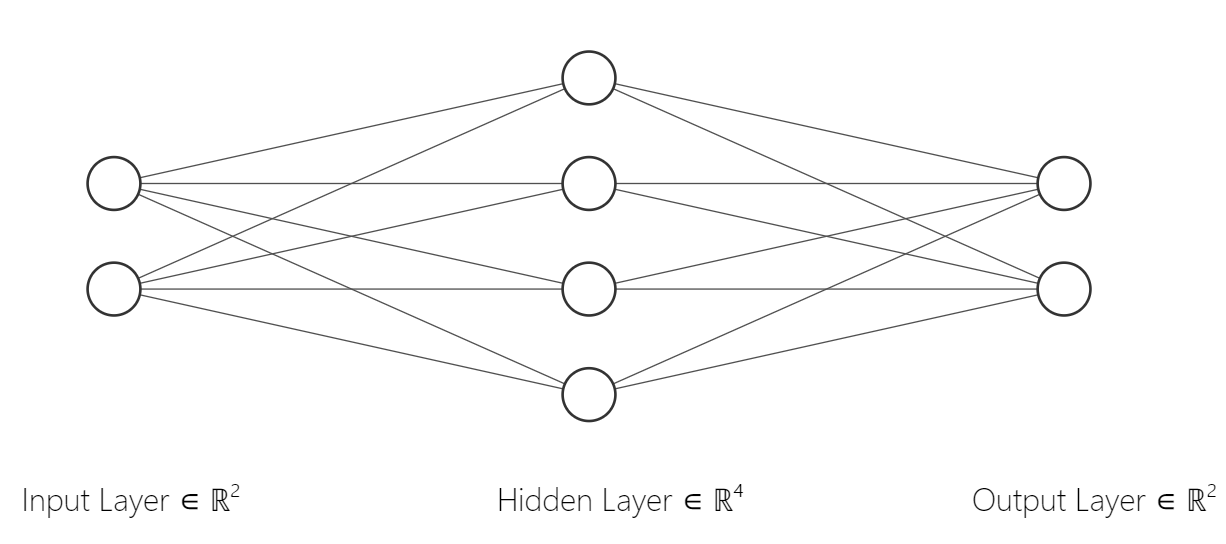
\includegraphics[width=0.7\textwidth]{../Images/neural_network_example.png}
    \caption{Neural network}
    \label{fig:neural_network}
\end{figure}

Deep neural networks are a type of neural network that is composed of multiple layers of neurons.
They are trained on a large dataset of images and then used to classify new images. There are countless architectures \cite{LIU201711} and implementations of neural networks, but they all share the same basic principles.



\subsection{Convolutional Neural Networks}

Convolutional Neural Networks (CNNs) are a type of neural network that is used for image recognition. They are used in a variety of applications, including self-driving cars, facial recognition, and medical imaging. They are trained on a large dataset of images and then used to classify new images. 


\subsection{Convolutional Neural Networks for source localization}

CNNs are mainly used to classify images but they can also classify sounds. They are used in this thesis to classify the spectrograms of the sound signals recorded by the microphone array. To do this, the spectrograms are converted into images and then fed into the CNN. The CNN then outputs a probability distribution over the possible classes. The class with the highest probability is then chosen as the predicted class.

\section{Related Work}

\subsection{}

